\documentclass[12pt,a4paper]{scrartcl}
\usepackage[utf8]{inputenc}
\usepackage[english,russian]{babel}
\usepackage{misccorr}
\usepackage{graphicx}
\usepackage{amsmath}
\usepackage{amsfonts}
\usepackage{verbatim}
\usepackage{listings}
\usepackage{pgfplots}
\usepackage{graphicx}
\usepackage{pdfpages}

\DeclareUnicodeCharacter{03BC}{\ensuremath{\mu}}

\usepackage{algorithm}
\usepackage{algpseudocode}

% Настройки листингов.
% 8 Листинги

\usepackage{listings}

% Значения по умолчанию
\lstset{
  language=[Sharp]C,
  basicstyle= \footnotesize,
  breakatwhitespace=true,% разрыв строк только на whitespacce
  breaklines=true,       % переносить длинные строки
%   captionpos=b,          % подписи снизу -- вроде не надо
  inputencoding=koi8-r,
  numbers=left,          % нумерация слева
  numberstyle=\footnotesize,
  showspaces=false,      % показывать пробелы подчеркиваниями -- идиотизм 70-х годов
  showstringspaces=false,
  showtabs=false,        % и табы тоже
  stepnumber=1,
  tabsize=4,              % кому нужны табы по 8 символов?
  frame=single,
  commentstyle=\color{green},
  morekeywords={partial, var, value, get, set},
  keywordstyle=\color{blue},
  stringstyle=\color{red}
}

% Стиль для псевдокода: строчки обычно короткие, поэтому размер шрифта побольше
\lstdefinestyle{pseudocode}{
  basicstyle=\small,
  keywordstyle=\color{black}\bfseries\underbar,
  language=Pseudocode,
  numberstyle=\footnotesize,
  commentstyle=\footnotesize\it
}

% Стиль для обычного кода: маленький шрифт
\lstdefinestyle{realcode}{
  basicstyle=\scriptsize,
  numberstyle=\footnotesize
}

% Стиль для коротких кусков обычного кода: средний шрифт
\lstdefinestyle{simplecode}{
  basicstyle=\footnotesize,
  numberstyle=\footnotesize
}

% Стиль для BNF
\lstdefinestyle{grammar}{
  basicstyle=\footnotesize,
  numberstyle=\footnotesize,
  stringstyle=\bfseries\ttfamily,
  language=BNF
}

% Определим свой язык для написания псевдокодов на основе Python
\lstdefinelanguage[]{Pseudocode}[]{Python}{
  morekeywords={each,empty,wait,do},% ключевые слова добавлять сюда
  morecomment=[s]{\{}{\}},% комменты {а-ля Pascal} смотрятся нагляднее
  literate=% а сюда добавлять операторы, которые хотите отображать как мат. символы
    {->}{\ensuremath{$\rightarrow$}~}2%
    {<-}{\ensuremath{$\leftarrow$}~}2%
    {:=}{\ensuremath{$\leftarrow$}~}2%
    {<--}{\ensuremath{$\Longleftarrow$}~}2%
}[keywords,comments]

% Свой язык для задания грамматик в BNF
\lstdefinelanguage[]{BNF}[]{}{
  morekeywords={},
  morecomment=[s]{@}{@},
  morestring=[b]",%
  literate=%
    {->}{\ensuremath{$\rightarrow$}~}2%
    {*}{\ensuremath{$^*$}~}2%
    {+}{\ensuremath{$^+$}~}2%
    {|}{\ensuremath{$|$}~}2%
}[keywords,comments,strings]

% Подписи к листингам на русском языке.
\renewcommand\lstlistingname{Листинг}
\renewcommand\lstlistlistingname{Листинги}


\begin{document}
\begin{titlepage}
\newpage
\begin{center}
Федеральное государственное бюджетное образовательное учреждение  \\
\vspace{0.25cm}%расстояние до верхней строчки
высшего образования «Московский государственный технический  \\
\vspace{0.25cm}%расстояние до верхней строчки
университет имени Н.Э.Баумана (национальный исследовательский \\
\vspace{0.25cm}%расстояние до верхней строчки
университет)» (МГТУ им. Н.Э.Баумана) \\
%\hrulefill %горизонтальная черта
\end{center}
\vspace{5cm}
\begin{center}
\Large Отчёт по лабораторной работе №1 \\ По дисциплине «Математическая статистика» \\ Тема: «Гистограмма и эмпирическая функция распределения» \\ Вариант: 1 % \\ означает перенос
\end{center}
%\vspace{2.5em}
\vspace{6em}
\begin{flushright}
Студент: \hrulefill Барсуков Н.М. \\
\vspace{1.5em}
Группа: \hrulefill ИУ7-66\\
\vspace{1.5em}
Преподаватель: \hrulefill Саркисян П.С.\\
\vspace{1.5em}
\end{flushright}
\vspace{\fill}
\begin{center}
Москва, 2020
\end{center}
\end{titlepage}
\newpage
\tableofcontents
\addcontentsline{toc}{section}{Введение}
\newpage
\begin{center}
\textbf {Введение}
\end{center}

Цель работы: построение гистограммы и эмпирической функции распределения.

Содержание работы:

Для выборки объёма n из генеральной совокупности X реализовать в виде программы на ЭВМ:
\begin{enumerate}
	\item вычисление максимального значения $M_{max}$ и минимального значения $M_{min}$;
	\item вычисление размаха R выборки;
	\item вычисление оценок $\hat{μ}$ и $S^2$ математического ожидания MX и дисперсии DX;
	\item группировку значений выборки в $m = [log_2 n] + 2$ интервала;
	\item построение на одной координатной плоскости гистограммы и графика функции плотности распределения вероятностей нормальной случайной величины с математическим ожиданием $\hat{μ}$ и дисперсией $S^2$;
	\item построение на одной координатной плоскости графика эмпирической функции распределения и функции распределения нормальной случайной величины с математическим ожиданием $\hat{μ}$ и дисперсией $S^2$.
\end{enumerate}

Провести вычисления и построить графики для выборки из индивидуального варианта.

\newpage
\addcontentsline{toc}{section}{Теоретическая часть}
\begin{center}
\textbf {Теоретическая часть}
\end{center}

Формулы для вычисления величин:
\begin{enumerate}
	\item максимальное значение \begin{equation}\label{eq1.1} M_{max} = max(x_1, x_2, ... , x_n) ;\end{equation}
	\item минимальное значение \begin{equation}\label{eq1.2}  M_{min} = min(x_1, x_2, ... , x_n) ;\end{equation} 
	\item размах выборки \begin{equation}\label{eq1.3} R = M_{max} - M_{min} ;\end{equation} 
	\item выборочное среднее \begin{equation}\label{eq1.4} \hat{μ} = \frac {1} {n} * \sum  \limits_{i=1}^n X_i ;\end{equation}
	\item несмещённая выборочная дисперсия \begin{equation}\label{eq1.5} S^2 = \frac {1} {(n - 1)} * \sum  \limits_{i=1}^n (X_i - \hat{μ})^2 . \end{equation} 
\end{enumerate}

Предположим, что для данной выборки $\overrightarrow {x_n}$ построили интервальный статистический ряд. Выберем некоторое m и разобьём отрезок $[x_{(1)}, x_{(n)}]$.

\underline {Определение}: эмпирической плотностью распределения, соответствующей реализации $\overrightarrow {x_n}$, называют функцию

\begin{equation}\label{eq1.6}
\begin{matrix}
f_n(x) & =
& \left\{
\begin{matrix}
\frac {n_i} {n * \Delta}, & \mbox{ } x \in J_i \\
0, & \mbox{ } x \notin J_i \\
\end{matrix} \right.
\end{matrix} .
\end{equation}

Интервалы:
\begin{equation}\label{eq1.7}
J = [x_{(1)},x_{(n)}] .
\end{equation}

Ширина интервалов
\begin{equation}\label{eq1.8}
\Delta = \frac {|J|} {m} ,
\end{equation}
где число интервалов
\begin{equation}\label{eq1.9}
m = [log_2n] + 2 .
\end{equation}

\begin{equation}\label{eq1.10}
J_i = [x_{(1)} + (i - 1) * \Delta, x_{(1)} + i * \Delta) , 
\end{equation}
где $i = \overline {1:m - 1}$.

\begin{equation}\label{eq1.11}
J_m = [x_{(1)} + (m - 1) * \Delta, x_{(1)} + m * \Delta] .
\end{equation}

$n_i$ - число элементов выборки, принадлежащих интервалу $J_i$, $i = \overline {1: m - 1}$.

\underline {Определение}: Гистограммой называется график этой вышеуказанной функции эмпирической плотности распределения.

Пусть $n(x, \overrightarrow {x_n})$ - количество элементов выборки $\overrightarrow {x_n}$, меньших $x$.

\underline {Определение}: Эмипирической функцией распределения, построенной по выборке $\overrightarrow {x_n}$, называется отображение $F_n: R \to R$ по правилу $F_n = \frac {n(x, \overrightarrow {x_n})} {n}$, где $n(x, \overrightarrow {x_n})$ - количество элементов выборки $\overrightarrow {x_n}$, которые имеют значение, меньшее $x$.

Если все элементы выборки $\overrightarrow {x_n}$ попарно различны, то

\begin{equation}\label{eq1.12}
\begin{matrix}
F_n & =
& \left\{
\begin{matrix}
0, &x \leq x_{(1)} \\
\frac {i} {n}, & \mbox{ } x \in (x_{(i)}, x_{(i+1)}], & i = \overline {1: n - 1} \\
1, & x  > x_{(n)}
\end{matrix} \right.
\end{matrix} .
\end{equation}

\newpage
\addcontentsline{toc}{section}{Листинг программы}
\begin{center}
\textbf {Листинг программы}
\end{center}

Текст программы $(labwork1.m)$:

\begin{verbatim}
function lab1()
	X = [-0.23,-1.03,-4.11,-0.65,-2.58,-0.79,-1.53,-0.18,-2.79,-1.97,-2.21,-1.59,-0.22,-3.18,-1.18,-1.42,-1.29,-2.22,-0.82,
	-1.87,-2.30,-0.94,-0.74,-2.45,-1.40,-2.09,-0.68,0.02,-1.80,-2.25,-1.19,-2.17,-1.89,-1.14,-1.50,-1.76,-0.69,-2.21,-1.65,
	-1.51,-2.11,-2.24,-0.72,0.94,-0.67,-2.44,-2.27,-1.33,-3.03,-0.42,-2.86,-2.00,-1.37,-1.90,-2.80,-0.89,-2.04,-1.66,-0.14,
	-2.79,-0.21,-1.29,-2.81,-0.29,-1.55,-0.45,-1.16,-3.96,-3.77,-3.36,-1.81,0.13,-2.61,-3.69,-3.00,-2.61,-0.74,-0.41,-0.78,
	-1.49,-1.89,-1.24,-0.00,-2.72,-1.69,-1.25,-1.59,0.20,-1.08,-2.42,-3.14,-2.54,-2.09,-2.51,-2.65,-2.42,-1.30,-0.65,1.40,
	-2.33,-1.97,-0.54,-1.13,-2.04,0.77,-1.03,-1.55,-1.47,-0.09,-2.11,-2.08,-1.79,-1.36,-1.92,-3.04,-1.08,-1.67,-2.11,-1.99,-1.64];
	X = sort(X);
	
	Mmax = max(X);
	Mmin = min(X);
	
	fprintf('Mmin = %s\n', num2str(Mmin));
	fprintf('Mmax = %s\n', num2str(Mmax));
	
	R = Mmax - Mmin;
	fprintf('R = %s\n', num2str(R));
	
	MU = getMU(X);
	fprintf('MU = %s\n', num2str(MU));
	
	Ssqr = getSsqr(X);
	fprintf('S^2 = %s\n', num2str(Ssqr));
	
	m = getNumberOfIntervals(X);
	fprintf('m = %s\n', num2str(m))
	
	createGroup(X);
	hold on;
	distributionDensity(X, MU, Ssqr, m);
	
	figure;
	empiricF(X);
	hold on;
	distribution(X, MU, Ssqr, m);
	end
	
	function mu = getMU(X)
	n = length(X);
	mu = sum(X)/n;
	end
	
function Ssqr = getSsqr(X)
	n = length(X);
	MX = getMU(X);
	Ssqr = sum((X - MX).^2) / (n-1);
	end
	
function m = getNumberOfIntervals(X)
	m = floor(log2(length(X)) + 2);
	end
	
function createGroup(X)
	n = length(X);
	m = getNumberOfIntervals(X);
	
	intervals = zeros(1, m+1);
	numCount = zeros(1, m+1);
	Delta = (max(X) - min(X)) / m;
	
	for i = 0: m
	intervals(i+1) = X(1) + Delta * i;
	end
	
	j = 1;
	count = 0;
	for i = 1:n
	if (X(i) >= intervals(j+1)) 
	j = j + 1; 
	end
	numCount(j) = numCount(j) + 1;
	count = count + 1;
	end
	
	graphBuf = numCount(1:m+1);
	for i = 1:m+1
	graphBuf(i) = numCount(i) / (n*Delta); 
	end
	
	stairs(intervals, graphBuf),grid;
	end
	
function distributionDensity(X, MX, DX, m)
	R = X(end) - X(1);
	delta = R/m;
	Sigma = sqrt(DX);
	
	Xn = (MX - R): delta/50 :(MX + R);
	Y = normpdf(Xn, MX, Sigma);
	plot(Xn, Y), grid;
	end
	
function distribution(X, MX, DX, m)
	R = X(end) - X(1);
	delta = R/m;
	
	Xn = (MX - R): delta :(MX + R);
	Y = 1/2 * (1 + erf((Xn - MX) / sqrt(2*DX))); 
	plot(Xn, Y, 'r'), grid;
	end
	
function empiricF(X)  
	[yy, xx] = ecdf(X);
	
	stairs(xx, yy), grid;
	end
\end{verbatim}

\newpage
\addcontentsline{toc}{section}{Результаты расчётов для выборки из индивидуального варианта}
\begin{center}
\textbf {Результаты расчётов для выборки из индивидуального варианта}
\end{center}

Для выборки согласно варианту были получены

\begin{enumerate}
	\item минимальное значение $M_{min} = -4.11$;
	\item максимальное значение $M_{max} = 1.400$;
	\item размах выборки $R = 5.510$;
	\item выборочное среднее $ \hat{μ} = -1.604583$;
	\item несмещённая выборочная дисперсия  $S^2 = 1.034091$.
\end{enumerate}

\begin{table}[ht]
	\caption{Интервальный ряд для индивидуального варианта}
	\begin{tabular}{|l|c|}
		\hline
		Интервал & Число\\
		\hline
		[-4.1100; -3.4213) & 4\\
		\hline
		[-3.4213; -2.7325) & 11\\
		\hline
		[-2.7325; -2.0438) & 26\\
		\hline
		[-2.0438; -1.3550) & 33\\
		\hline
		[-1.3550; -0.6663) & 26\\
		\hline
		[-0.6663; 0.0225) & 15\\
		\hline
		[0.0225; 0.7112) & 2\\
		\hline
		[0.7112; 1.4000] & 3\\
		\hline
	\end{tabular}
	\label{tab:tabular}
\end{table}

В результате проведённых вычислений были получены два графика. На графике \ref{graph2.1} представлены гистограмма и функция плотности распределения нормальной величины, на графике \ref{graph2.2} - эмпирическая функция распределения и функция распределения нормальной случайной величины.

\begin{figure}
	\centering
	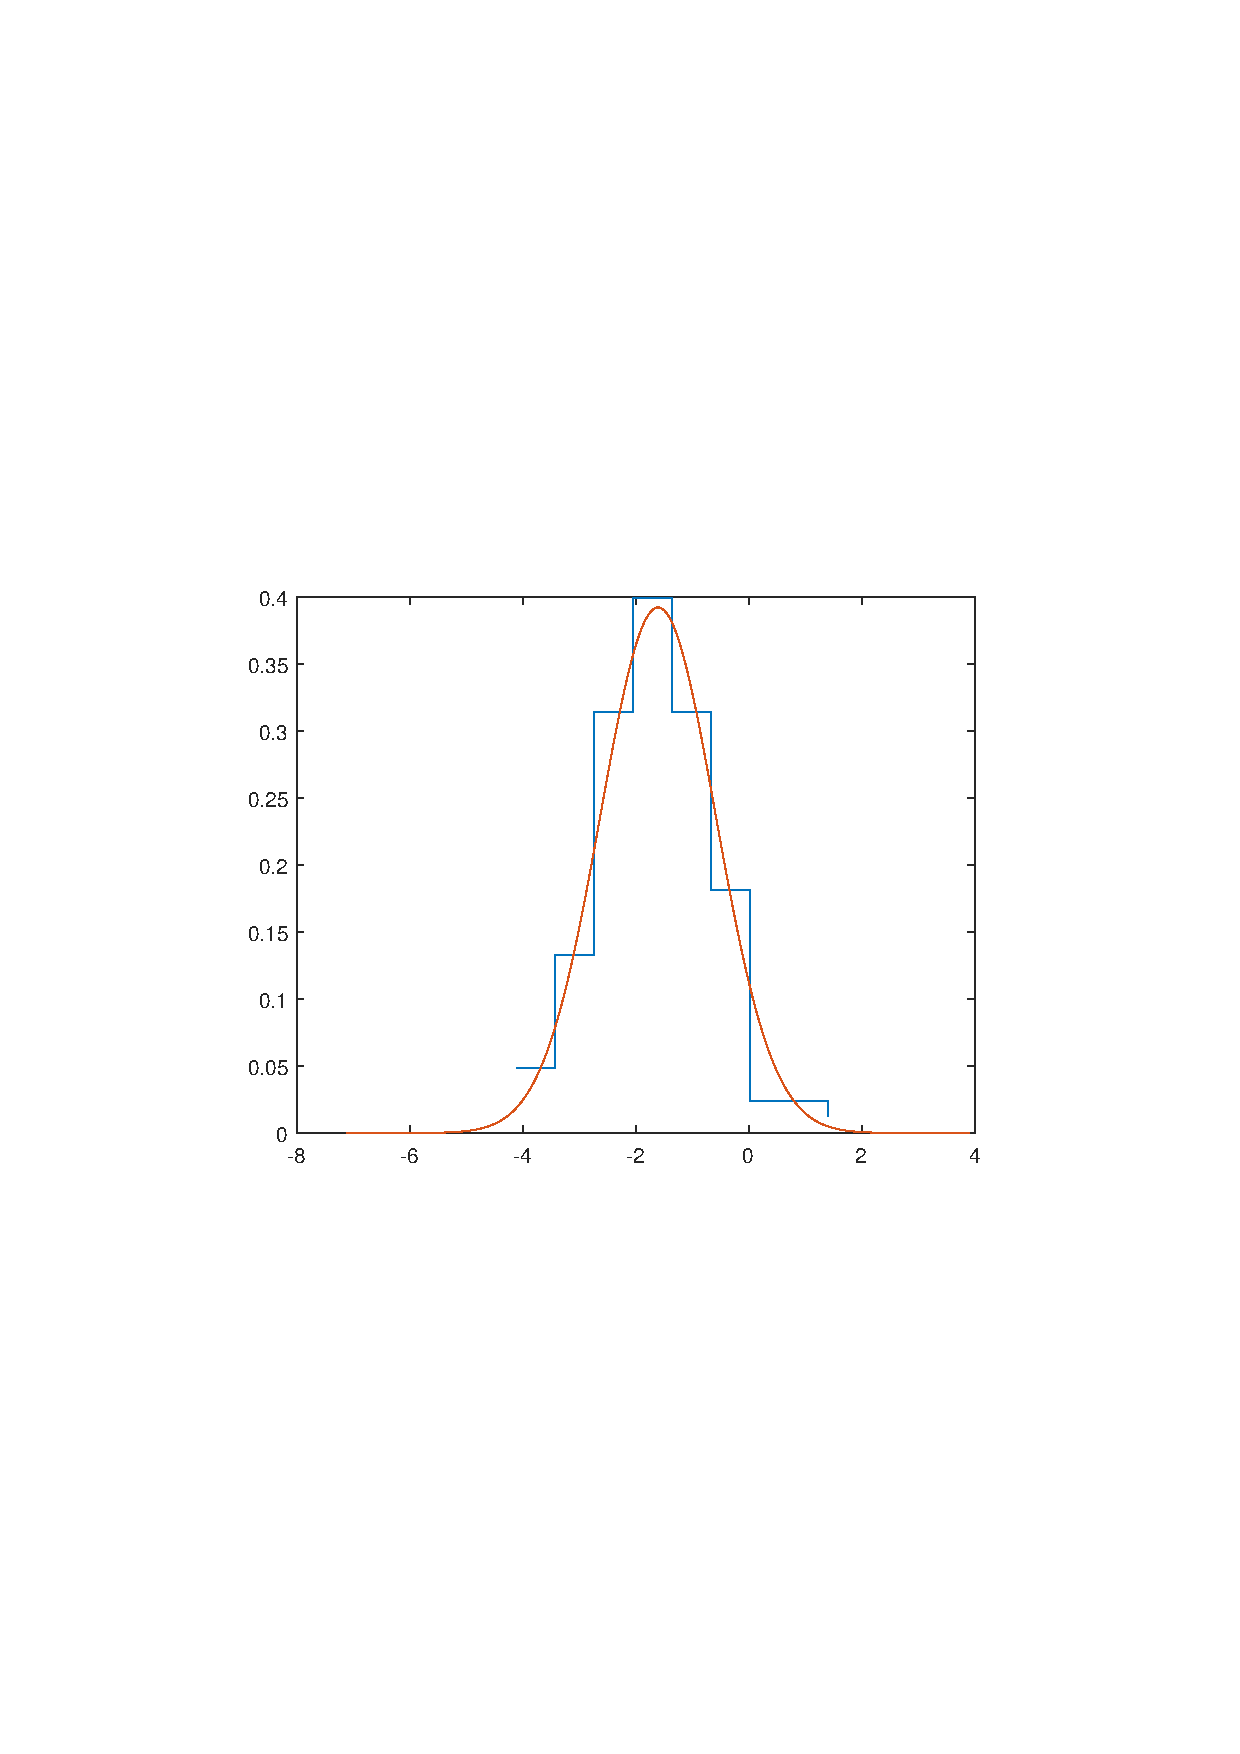
\includegraphics[width=1\linewidth]{2}
	\caption{Гистограмма  и график функции плотности распределения нормальной случайной величины}
	\label{graph2.2}
\end{figure}

\begin{figure}
	\centering
	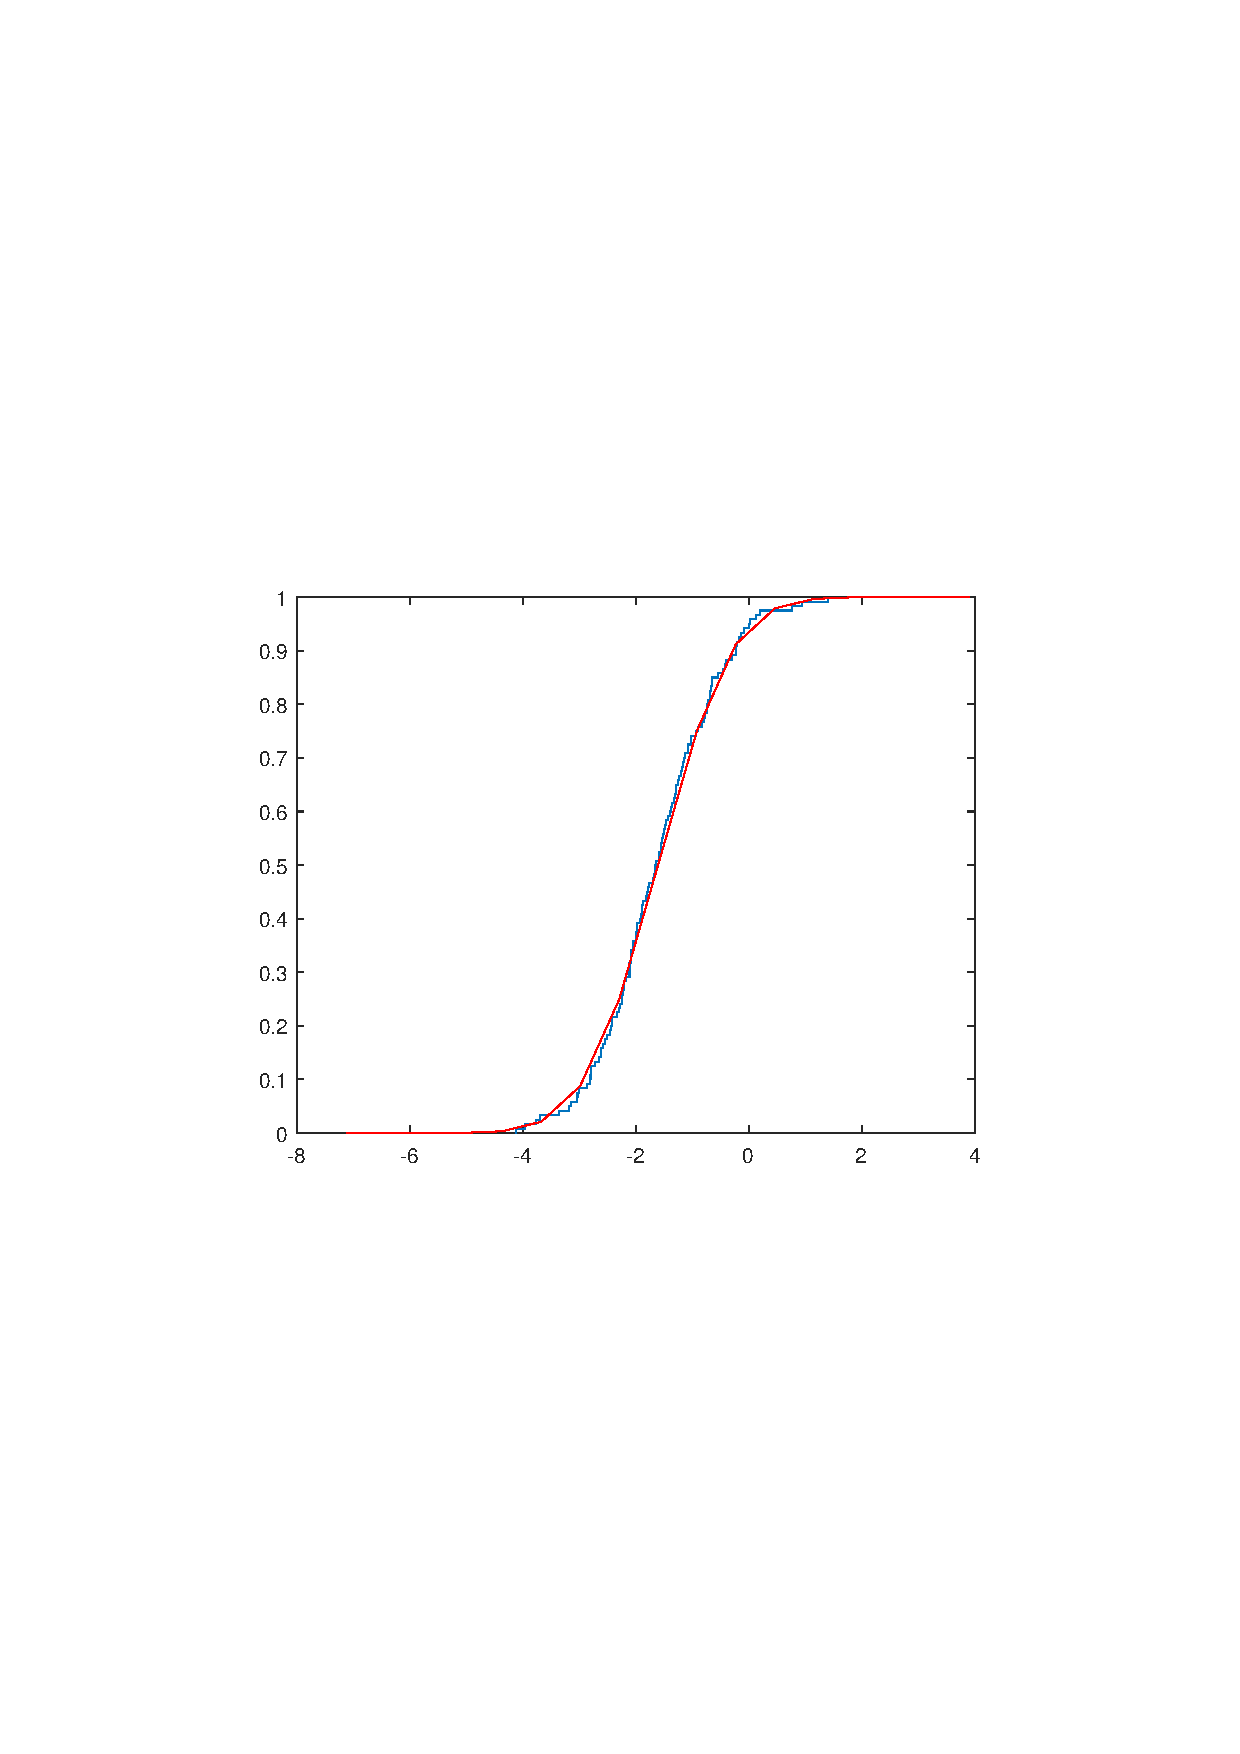
\includegraphics[width=1\linewidth]{1}
	\caption{График эмпирической функции распределения и функции распределения нормальной случайной величины}
	\label{graph2.1}
\end{figure}

\newpage
\addcontentsline{toc}{section}{Заключение}
\begin{center}
\textbf {Заключение}
\end{center}
В результате выполнения лабораторной работы для заданной согласно варианту выборки были получены гистограмма и эмпирическая функция распределения. Для выполнения вычислений был написан код MatLab, позволяющий вычислить интервальный ряд распределения, минимальное и максимальное значения, размах выборки, выборочное среднее, несмещённую выборочную дисперсию.

\end{document}